\documentclass[]{article}
\usepackage[top=1.5in,bottom=1.5in,left=1in,right=1in]{geometry}
\usepackage{tikz}
\usetikzlibrary{shapes.geometric}
\usepackage{subcaption}
\usepackage{xcolor}
\usepackage[colorlinks,allcolors=blue]{hyperref}
\usepackage[noabbrev]{cleveref}


\newcommand{\gameName}{Expendibots}

\title{
    {\LARGE Rules for the Game of}
    \\[1ex]
    {\Huge\bf \gameName}
}
\author{
    \textbf{Adam Kues}
    and
    \textbf{Matthew Farrugia-Roberts}
    \\
    \textit{The University of Melbourne}
    \\
    Contact: \href
      {mailto:matt.farrugia@unimelb.edu.au}
      {\tt matt.farrugia@unimelb.edu.au}
}
\date{2020}


% Custom TikZ commands
\newcommand{\white}[3] {
    \foreach \x in {1,...,#3}
        \node[draw,thick,minimum size=17,fill=black!30,circle]
            at ({.5+#1},{\x*.1+.4+#2}) {};
    \node[draw,thick,minimum size=17,fill=white,circle]
        at ({.5+#1},{#3*.1+.5+#2}) {};
    \node[]
        at ({.5+#1},{#3*.1+.5+#2}) {\large #3};
}
\newcommand{\black}[3] {
    \foreach \x in {1,...,#3}
        \node[draw,thick,minimum size=15,fill=black!60,rounded corners=0.6mm]
            at ({.5+#1},{\x*.1+.4+#2}) {};
    \node[draw,thick,minimum size=15,fill=black!30,rounded corners=0.6mm]
        at ({.5+#1},{#3*.1+.5+#2}) {};
    \node[]
        at ({.5+#1},{#3*.1+.5+#2}) {\large #3};
}
\newcommand{\colorSquare}[3] {
  \draw[fill=#1] ({#2},{#3}) rectangle ({#2+1},{#3+1});
}
\newcommand{\board} {
    \tikzset{
        x=0.8cm,
        y=0.8cm,
    }
    \draw[fill=black!5,very thick] (0, 0) rectangle (8, 8);
    \draw[step=1] (0, 0) grid (8, 8);
}

\begin{document}

\maketitle

\begin{quote}
    \emph{\gameName} is a fast paced action game where assembling and
    disassembling powerful stacks of bots will be the key to your survival.
    Sneak behind enemy lines and cause chain reactions to do huge damage,
    but watch out for friendly fire!
    Can you successfully fend off your opponent's attacks and emerge
    victorious?
\end{quote}

\section*{Setup}

\emph{\gameName} is played on a $8 \times 8$ board consisting of 64
\textbf{squares}, as illustrated in \Cref{fig:board}. Two \textbf{players},
\textbf{White} and \textbf{Black}, play the game.
%
Each player initially controls 12 \textbf{tokens} of their own colour.
The pieces begin in the configuration shown below in \Cref{fig:board},
occupying the back two rows in 3 square formations.
%
One or more tokens of the same colour on a single square form a
\textbf{stack}; for ease of rendering in 2D, we depict the number
of tokens in a stack by a number placed on the token in the diagram.
%
In the initial position, all stacks are of size 1 (a single token).
There is no limit to the number of tokens in a stack.

\begin{figure}[ht!]
    \centering
    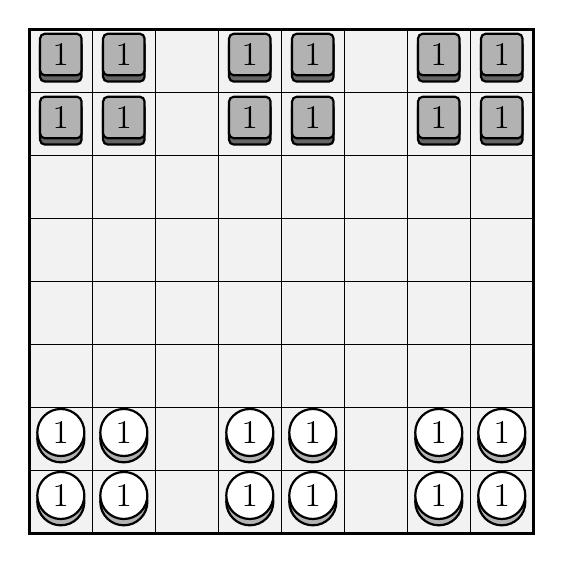
\begin{tikzpicture}
        \board
        \white{0}{0}{1};
        \white{0}{1}{1};
        \white{1}{0}{1};
        \white{1}{1}{1};
        \white{3}{0}{1};
        \white{3}{1}{1};
        \white{4}{0}{1};
        \white{4}{1}{1};
        \white{6}{0}{1};
        \white{6}{1}{1};
        \white{7}{0}{1};
        \white{7}{1}{1};
        \black{0}{6}{1};
        \black{0}{7}{1};
        \black{1}{6}{1};
        \black{1}{7}{1};
        \black{3}{6}{1};
        \black{3}{7}{1};
        \black{4}{6}{1};
        \black{4}{7}{1};
        \black{6}{6}{1};
        \black{6}{7}{1};
        \black{7}{6}{1};
        \black{7}{7}{1};
    \end{tikzpicture}
    \caption{
    \label{fig:board}
        Board and initial starting configuration of 24~tokens (12~White,
        12~Black)
    }
\end{figure}

\newpage

\section*{Gameplay}

Players alternate taking turns, with White having the first turn.
This cycle repeats until the game ends. On each turn, the current
player must take a single \textbf{action} involving a stack of their
colour. This action may be a \textbf{move action} or a
\textbf{boom action}. Each type of action is described in the
following sections.

\subsection*{Move actions}

A \textbf{move action} (a `move') involves moving \emph{some} or \emph{all}
of the tokens in a stack some number of squares in one of the four
\emph{cardinal directions} (up, down, left, or right).
From a stack of $n$ tokens ($n \geq 1$), the player may move up to $n$ of
those tokens a distance of up to $n$ squares in a single direction.
The tokens may \emph{not} move diagonally, and must move by at least one
square.
%
The destination square may be unoccupied, or it may already be occupied by
tokens of the same colour---in this case, the moved tokens join the tokens
on the destination square, forming a new stack whose number of tokens is
equal to the number of tokens originally on the square plus the number of
tokens moved onto the square.
%
The tokens may \emph{not} move onto a square occupied by the opponent's
tokens. However, the tokens may move `over' it (as long as the total
distance moved is not more than $n$ squares). A token cannot move off the
board.

\begin{figure}[ht!]
\centering
\begin{subfigure}{.45\textwidth}
    \centering
    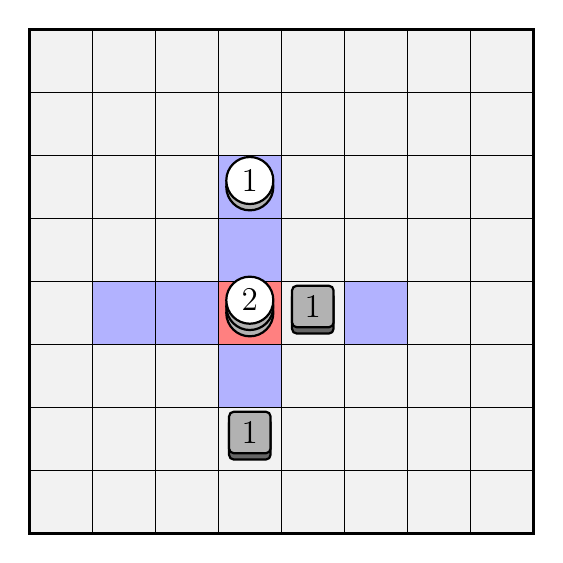
\begin{tikzpicture}
        \board
        \colorSquare{white!50!red}{3}{3};
        \colorSquare{white!70!blue}{1}{3};
        \colorSquare{white!70!blue}{2}{3};
        \colorSquare{white!70!blue}{5}{3};
        \colorSquare{white!70!blue}{3}{2};
        \colorSquare{white!70!blue}{3}{4};
        \colorSquare{white!70!blue}{3}{5};
        \white{3}{3}{2};
        \white{3}{5}{1};
        \black{3}{1}{1};
        \black{4}{3}{1};
    \end{tikzpicture}
    \caption{\label{fig:move-1}
        The stack marked with red has 2 tokens.
        Thus, the player may move one or both of these tokens
        up to 2 squares in any of the cardinal directions.
        The player has 12 possible move actions it could take with
        this stack---moving 1 or 2 tokens to any of the 6 squares marked in
        blue.
        Note that the squares already occupied with opposing tokens cannot be
        the destination for this move.
    }
\end{subfigure}
\begin{subfigure}{.01\textwidth}
\phantom{SP}
\end{subfigure}
\begin{subfigure}{.51\textwidth}
    \centering
    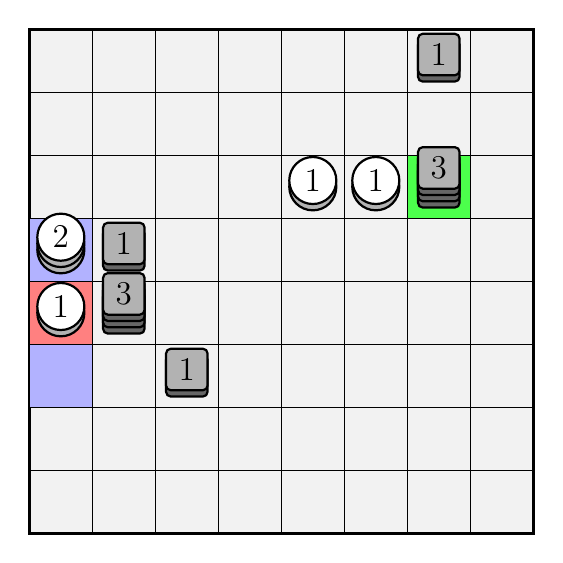
\begin{tikzpicture}
        \board
        \colorSquare{white!50!red}{0}{3};
        \colorSquare{white!70!blue}{0}{4};
        \colorSquare{white!70!blue}{0}{2};
        \colorSquare{white!30!green}{6}{5};
        \white{0}{3}{1};
        \white{0}{4}{2};
        \black{1}{4}{1};
        \black{1}{3}{3};
        \black{2}{2}{1};
        \black{6}{5}{3};
        \white{5}{5}{1};
        \white{4}{5}{1};
        \black{6}{7}{1};
    \end{tikzpicture}
    \caption{\label{fig:move-2}
        The stack marked with red only consists of a single token, so it
        can only move a single square in the cardinal directions.
        It cannot move off the board or onto a stack of a different colour,
        so it can only has 2 possible moves (to the squares marked in blue).
        If it were to move up, the square above would then have a single
        white stack of 3 tokens.
        Quiz: The stack marked in green has 21 distinct move actions it
        could make---can you find them all?
    }
\end{subfigure}
\caption{\label{fig:moves}
    Two different scenarios for understanding the move action.
}
\end{figure}

\newpage

\subsection*{Boom actions}

A \textbf{boom action} (a `boom') involves choosing a stack to
\emph{explode}. All of the tokens in this stack are removed from play as a
result of this explosion.
% 
Additionally, the explosion immediately causes any stacks (of either color)
in a $3 \times 3$ square area surrounding this stack to also explode.
These explosions may go on to trigger further explosions in a recursive
chain reaction.
In this way, long chains of stacks may be removed from play as the result
of a single action.

\begin{figure}[ht!]
\centering
\begin{subfigure}{.37\textwidth}
    \centering
    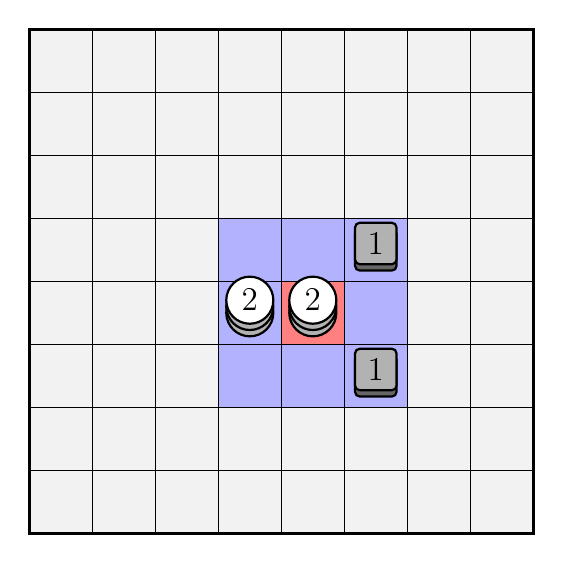
\begin{tikzpicture}
        \board
        \colorSquare{white!50!red}{4}{3};
        \colorSquare{white!70!blue}{5}{2};
        \colorSquare{white!70!blue}{3}{2};
        \colorSquare{white!70!blue}{5}{3};
        \colorSquare{white!70!blue}{3}{3};
        \colorSquare{white!70!blue}{5}{4};
        \colorSquare{white!70!blue}{3}{4};
        \colorSquare{white!70!blue}{4}{4};
        \colorSquare{white!70!blue}{4}{2};
        \white{3}{3}{2};
        \white{4}{3}{2};
        \black{5}{4}{1};
        \black{5}{2}{1};
    \end{tikzpicture}
    \caption{\label{fig:radius}
        If the White player chooses to explode the stack marked in red, all
        the tokens in the $3 \times 3$ square blue zone will also explode.
        In this case, this would result in the removal of all tokens on the
        board.
        \vspace{2\baselineskip}
    }
\end{subfigure}
\begin{subfigure}{.01\textwidth}
\phantom{SP}
\end{subfigure}
\begin{subfigure}{.60\textwidth}
    \centering
    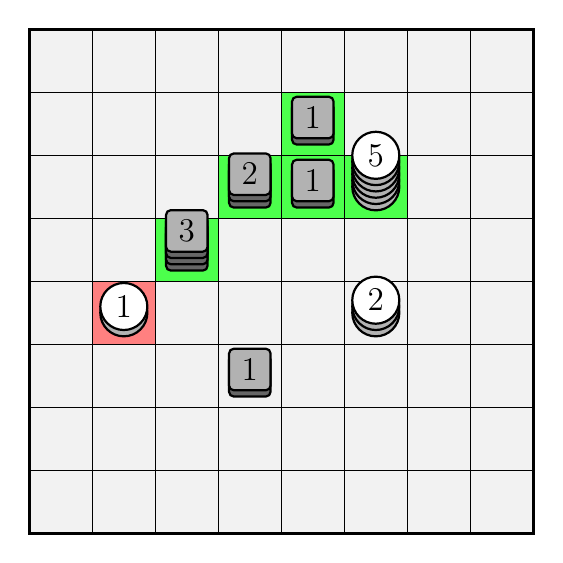
\begin{tikzpicture}
        \board
        \colorSquare{white!50!red}{1}{3};
        \colorSquare{white!30!green}{2}{4};
        \colorSquare{white!30!green}{3}{5};
        \colorSquare{white!30!green}{4}{5};
        \colorSquare{white!30!green}{4}{6};
        \colorSquare{white!30!green}{5}{5};
        \white{1}{3}{1};
        \black{2}{4}{3};
        \black{3}{5}{2};
        \black{4}{5}{1};
        \black{4}{6}{1};
        \white{5}{5}{5};
        \white{5}{3}{2};
        \black{3}{2}{1};
    \end{tikzpicture}
    \caption{\label{fig:chain}
        If the White player chooses to explode the stack marked in red, the Black 3-stack
    will be caught in the explosion. This 3-stack will also explode, causing the Black 2-stack
    to explode, followed by the nearby Black 1-stacks, and finally the White 5-stack.
        This would result in all the stacks marked in red or green to be removed from play.
        The White 2-stack and the lowermost Black 1-stack are not in the range of any of the
        explosions, so they would not be affected by the action.
    }
\end{subfigure}
\caption{\label{fig:boom}
    Two different scenarios for understanding the boom action.
}
\end{figure}

\section*{Ending the game}

The game ends as soon as at least one player has no remaining tokens.
At this point, the player who still has at least one token is declared
the winner.
If both players lose their remaining tokens simultaneously, the game is
declared a draw.
A draw is also declared if either of the following conditions are met:

\begin{itemize}
    \item
        One board configuration (with all stacks in the same position and
        quantity) occurs for a fourth time since the start of the game.
        These repeated board configurations do not need to occur in
        succession.
    \item
        Each player has had their 250\textsuperscript{th} turn without
        a winner being declared.
\end{itemize}

\end{document}
